\section{Logistic Regression} \label{logistic}
This section describes attempt to predict the condition status of the water pump by means of multinomial logistic regression (MLR). The model was fit using \texttt{multinom} function from the \texttt{nnet} package in R to perform MLR. The package uses feed-forward neural networks with a single hidden-layer and \texttt{multinom} function fits multinomial log-linear models. MLR is an extension of a simple logistic regression that allows for predicting variables with three or more categories. 

The target categorical variables are \textsc{functional, functional needs repair,} and \textsc{non functional} which correspond to the status of the water pump's condition. Prior to fitting the model, the data was split in the ratio of $1/3$ and $2/3$ to create training and test datasets, respectively. 

The initial model included all the features and the accuracy rate for training data and testing data were 73.41$\%$ and 72.68$\%$, respectively. When applied to the whole training, the accuracy rate was 73.22$\%$. After submitting the predictions to the competition website we got the score of 71.43$\%$. Below is the confusion matrix associated with this model:

\begin{figure}[h]
    \centering
    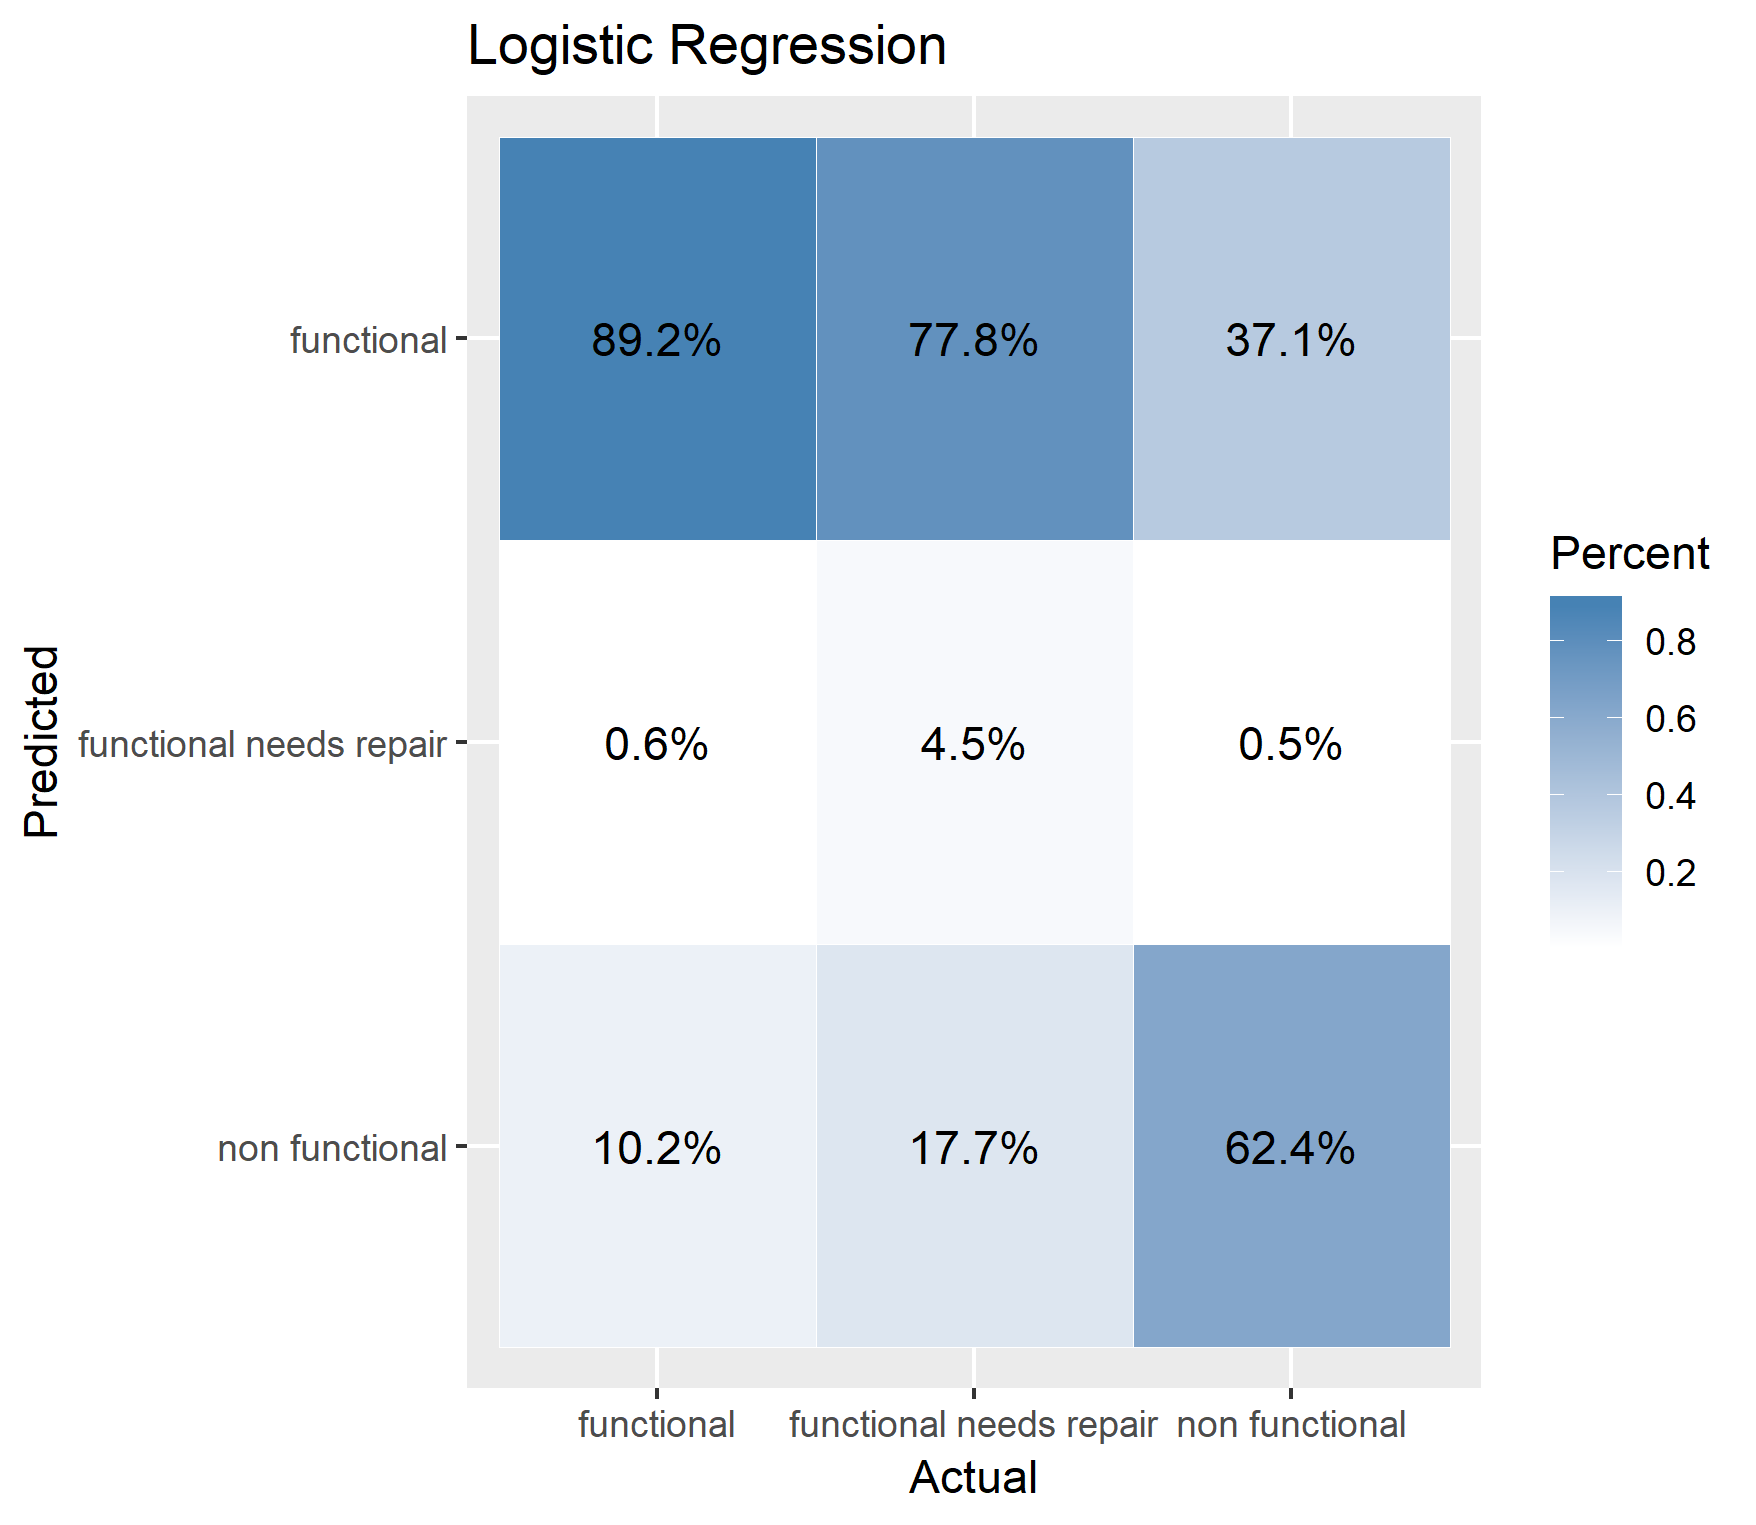
\includegraphics[width=0.6\textwidth]{Figures/LogConfMatrix.png}
    \caption{Confusion matrix for the logistic regression model.}
    \label{fig:NonNormalHists}
\end{figure}

The confusion matrix indicates that most of the inaccuracy is associated with miss-classification of the \textsc{functional needs repair} category with 95.5$\%$ overall error rate where 77.8$\%$ of this class is miss-classified as \textsc{functional} and 17.7$\%$ as \textsc{non functional}. The \textsc{non functional} category is the second most inaccurately classified category with 37.6$\%$ error rate where 37.1$\%$ of this class is miss-classified as \textsc{functional}. Lastly, only 10.8$\%$ of functional pumps were miss-classified. 

Further, the prediction accuracy was compared among several models with varying features and interactions between certain features, which seemed to perform better on the training data. The best rate recorded for the training data was equal to 73.68$\%$. However, after comparing the accuracy rates for the test data, it was found that the prediction accuracy did not differ between these models. The highest submission score achieved after all these attempts indicated 72.11$\%$ accuracy.  
